% Options for packages loaded elsewhere
\PassOptionsToPackage{unicode}{hyperref}
\PassOptionsToPackage{hyphens}{url}
\documentclass[
]{article}
\usepackage{xcolor}
\usepackage[margin=1in]{geometry}
\usepackage{amsmath,amssymb}
\setcounter{secnumdepth}{5}
\usepackage{iftex}
\ifPDFTeX
  \usepackage[T1]{fontenc}
  \usepackage[utf8]{inputenc}
  \usepackage{textcomp} % provide euro and other symbols
\else % if luatex or xetex
  \usepackage{unicode-math} % this also loads fontspec
  \defaultfontfeatures{Scale=MatchLowercase}
  \defaultfontfeatures[\rmfamily]{Ligatures=TeX,Scale=1}
\fi
\usepackage{lmodern}
\ifPDFTeX\else
  % xetex/luatex font selection
\fi
% Use upquote if available, for straight quotes in verbatim environments
\IfFileExists{upquote.sty}{\usepackage{upquote}}{}
\IfFileExists{microtype.sty}{% use microtype if available
  \usepackage[]{microtype}
  \UseMicrotypeSet[protrusion]{basicmath} % disable protrusion for tt fonts
}{}
\makeatletter
\@ifundefined{KOMAClassName}{% if non-KOMA class
  \IfFileExists{parskip.sty}{%
    \usepackage{parskip}
  }{% else
    \setlength{\parindent}{0pt}
    \setlength{\parskip}{6pt plus 2pt minus 1pt}}
}{% if KOMA class
  \KOMAoptions{parskip=half}}
\makeatother
\usepackage{longtable,booktabs,array}
\usepackage{calc} % for calculating minipage widths
% Correct order of tables after \paragraph or \subparagraph
\usepackage{etoolbox}
\makeatletter
\patchcmd\longtable{\par}{\if@noskipsec\mbox{}\fi\par}{}{}
\makeatother
% Allow footnotes in longtable head/foot
\IfFileExists{footnotehyper.sty}{\usepackage{footnotehyper}}{\usepackage{footnote}}
\makesavenoteenv{longtable}
\usepackage{graphicx}
\makeatletter
\newsavebox\pandoc@box
\newcommand*\pandocbounded[1]{% scales image to fit in text height/width
  \sbox\pandoc@box{#1}%
  \Gscale@div\@tempa{\textheight}{\dimexpr\ht\pandoc@box+\dp\pandoc@box\relax}%
  \Gscale@div\@tempb{\linewidth}{\wd\pandoc@box}%
  \ifdim\@tempb\p@<\@tempa\p@\let\@tempa\@tempb\fi% select the smaller of both
  \ifdim\@tempa\p@<\p@\scalebox{\@tempa}{\usebox\pandoc@box}%
  \else\usebox{\pandoc@box}%
  \fi%
}
% Set default figure placement to htbp
\def\fps@figure{htbp}
\makeatother
\setlength{\emergencystretch}{3em} % prevent overfull lines
\providecommand{\tightlist}{%
  \setlength{\itemsep}{0pt}\setlength{\parskip}{0pt}}
\usepackage{bookmark}
\IfFileExists{xurl.sty}{\usepackage{xurl}}{} % add URL line breaks if available
\urlstyle{same}
\hypersetup{
  pdftitle={Global Patterns in Climate Awareness, COVID-19 Impact, and National Happiness},
  pdfauthor={Put your group name here: The Geese},
  hidelinks,
  pdfcreator={LaTeX via pandoc}}

\title{Global Patterns in Climate Awareness, COVID-19 Impact, and National Happiness}
\usepackage{etoolbox}
\makeatletter
\providecommand{\subtitle}[1]{% add subtitle to \maketitle
  \apptocmd{\@title}{\par {\large #1 \par}}{}{}
}
\makeatother
\subtitle{Exploring Disparate Data: Part 3 - Final Report}
\author{Put your group name here: The Geese}
\date{Due November 26th, 2025}

\begin{document}
\maketitle

List your group members, including their student numbers, here:
- Sophia Thai (\#169112540)
- Kaya Darling(\#169112257)

\section{Data Description}\label{data-description}

\subsection{Climate Change Awareness Data}\label{climate-change-awareness-data}

\begin{verbatim}
## # A tibble: 110 x 7
##    country         aware_no aware_alittle aware_moderate aware_alot aware_refuse
##    <chr>              <dbl>         <dbl>          <dbl>      <dbl>        <dbl>
##  1 Albania             9.99          43.0           33.1      10.6         3.25 
##  2 Algeria            23.2           37.6           26.0      11.1         2.15 
##  3 Angola             19.1           43.0           23.5      11.1         3.29 
##  4 Argentina           8.25          37.4           43.8       9.88        0.696
##  5 Armenia             9.18          51.4           25.8      11.4         2.14 
##  6 Asian & Pacifi~    13.3           40.1           24.8      19.5         2.26 
##  7 Australia           1.13          26.4           48.1      23.9         0.407
##  8 Austria             1.34          16.4           48.6      32.7         0.985
##  9 Azerbaijan          6.19          42.4           35.9      13.2         2.20 
## 10 Bangladesh         24.5           36.2           16.2      18.9         4.22 
## # i 100 more rows
## # i 1 more variable: aware_base <dbl>
\end{verbatim}

The data come from HDX (Humanitarian Data Exchange) and describes the responses to a survey in 2022 from the Meta Climate Change Opinion Survey. This survey asked people in many different countries their level of awareness on climate change and recorded their responses \footnote{Meta. (2022). Meta Climate Change Opinion Survey 2022 {[}Data set{]}. Humanitarian Data Exchange (HDX). \url{https://data.humdata.org/dataset/meta-climate-change-opinion-survey}}. The people doing the survey had the option to choose between different statements that represented their awareness of climate change. For example, if they we not aware at all the participant would select ``I have never heard of it''.

In order to clean the data, we first adjusted so that all of the periods in between name were removed and replaced with spaces. Then, we adjusted the country names that were called something different from their name in the other data sets to match the other data sets country names. This was to ensure that in joining everything goes smoothly.

\subsection{Covid 2020 Cases Data}\label{covid-2020-cases-data}

The data come from the Our World in Data COVID\_19 database and detail the number of covid cases in each country in 2020, recorded daily \footnote{Ritchie, H., Mathieu, E., Rodés-Guirao, L., Appel, C., Giattino, C., Ortiz-Ospina, E., Hasell, J., Macdonald, B., Beltekian, D., \& Roser, M. (2020). Coronavirus pandemic (COVID-19) {[}Data set{]}. Our World in Data. \url{https://ourworldindata.org/coronavirus}}.

In order to clean the data, we adjusted some of the names to match the climate awareness data by changing some of the names of certain countries so that they all match.

\subsection{World Happiness Report Data}\label{world-happiness-report-data}

This data comes from the World Happiness Report from 2023 and detail how people responded to a question about the ``Life Ladder'' \footnote{Helliwell, J. F., Layard, R., Sachs, J. D., \& De Neve, J.-E. (2023). World Happiness Report 2023 {[}Data set{]}. Sustainable Development Solutions Network. \url{https://worldhappiness.report}} about how they rate their overall life satisfaction from 0 to 10. The data has the overall well being of a country depending on how participants from these countries rated their life on the ladder.

In order to clean the data, we didn't have to do any cleaning, as it was already clean from part 1!

\subsection{Combining the Data}\label{combining-the-data}

We first joined climate awareness data to covid data by selecting only columns ``country'', ``continent'', and \texttt{total\textbackslash{}\_cases}. Then, we used \texttt{inner\textbackslash{}\_join} to join those columns of the covid 2020 data with the climate awareness data.

For combining happiness data with climate awareness and covid data, we joined this data to the data set \texttt{climate\textbackslash{}\_covid}, which was made from joining the previous two data sets. We used \texttt{inner\textbackslash{}\_join()} to join the columns \texttt{"country"} and \texttt{"ladder\textbackslash{}\_score"} from the happiness data to the climate awareness and covid data.

\section{Exploratory Data Analysis}\label{exploratory-data-analysis}

To achieve our goals, we explored the data by\ldots{}

We explored many aspects of the data, but will demonstrate three. These are: in countries with higher covid cases there are more people reporting high climate awareness, countries with higher climate awareness are happier, and countries with higher covid cases are also happier

The first aspect that we found interesting is shown in this scatterplot. The insight should be specific to the data shown, not a general statement beyond the data (leave that for the conclusion).

\pandocbounded{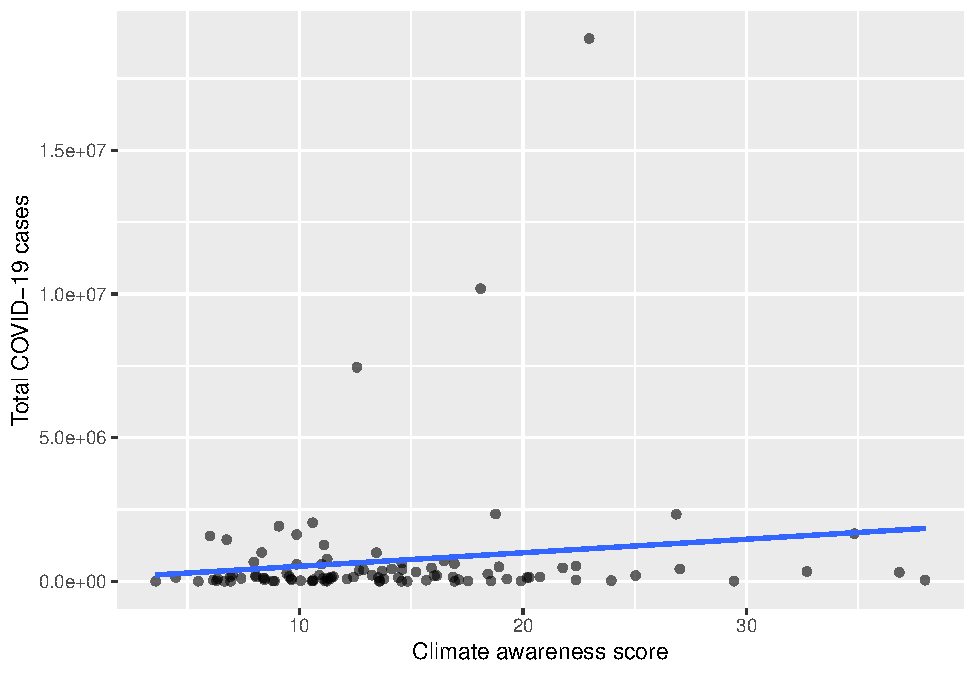
\includegraphics[keepaspectratio]{DATA100Assignment3PartII_Final_Report_Template_files/figure-latex/insight1-1.pdf}}
We observe a positive relationship between the percentage of respondents who reported ``I know a lot about climate change'' and the total number of COVID-19 cases \footnote{Meta. (2022). Meta Climate Change Opinion Survey 2022 {[}Data set{]}. Humanitarian Data Exchange (HDX). \url{https://data.humdata.org/dataset/meta-climate-change-opinion-survey}}\footnote{Ritchie, H., Mathieu, E., Rodés-Guirao, L., Appel, C., Giattino, C., Ortiz-Ospina, E., Hasell, J., Macdonald, B., Beltekian, D., \& Roser, M. (2020). Coronavirus pandemic (COVID-19) {[}Data set{]}. Our World in Data. \url{https://ourworldindata.org/coronavirus}}. This pattern does not imply that climate awareness causes higher case counts; rather, it reflects broader national characteristics. Countries with stronger education systems and greater access to information tend to show higher levels of climate awareness. These same countries also typically have higher population densities, more international travel, and more comprehensive COVID-19 testing and reporting infrastructure. Together, these factors produce the positive trend observed in the data.

This insight is supported by the summary statistics in table @ref(tab:summary\_stats)

\begin{tabular}{l|r}
\hline
metric & correlation\\
\hline
Correlation & 0.144\\
\hline
\end{tabular}

The next insight that we found is shown in \ref{fig:insight2}.

\begin{figure}
\centering
\pandocbounded{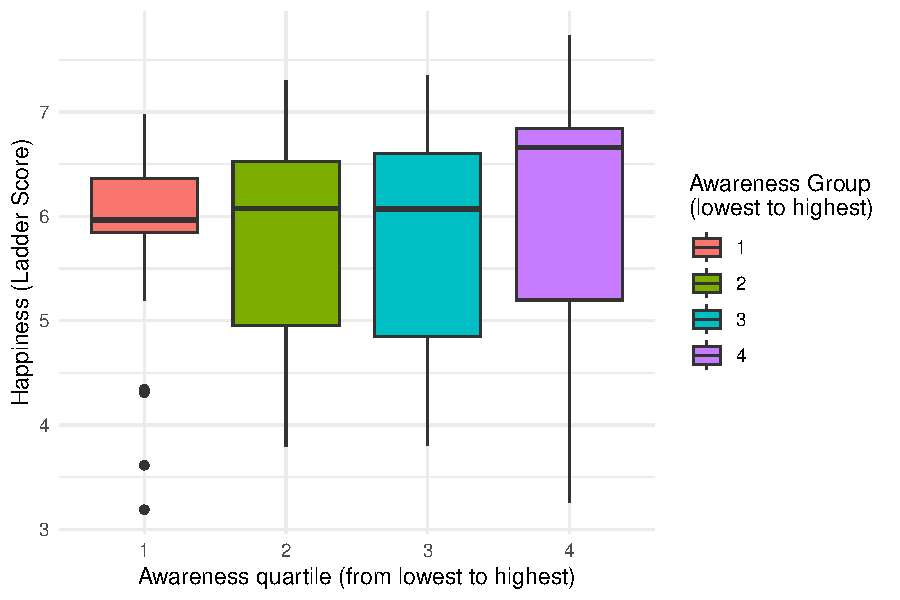
\includegraphics[keepaspectratio]{DATA100Assignment3PartII_Final_Report_Template_files/figure-latex/insight2-1.pdf}}
\caption{\label{fig:insight2}Happiness scores by climate awareness quartile}
\end{figure}

Countries with greater climate awareness tend to have higher reported happiness scores, based on data from the Meta Climate Change Survey and the World Happiness Report \footnote{Meta. (2022). Meta Climate Change Opinion Survey 2022 {[}Data set{]}. Humanitarian Data Exchange (HDX). \url{https://data.humdata.org/dataset/meta-climate-change-opinion-survey}}\footnote{Ritchie, H., Mathieu, E., Rodés-Guirao, L., Appel, C., Giattino, C., Ortiz-Ospina, E., Hasell, J., Macdonald, B., Beltekian, D., \& Roser, M. (2020). Coronavirus pandemic (COVID-19) {[}Data set{]}. Our World in Data. \url{https://ourworldindata.org/coronavirus}}.

This boxplot shows a clear upward trend, indicating that countries with greater climate awareness tend to have higher reported happiness scores. This pattern likely reflects broader structural differences rather than a direct causal relationship. Countries with higher climate awareness often also have better access to education, higher GDP, more stable institutions, and stronger scientific and media communication systems. These underlying factors contribute both to increased awareness of climate issues and to higher Life Ladder scores, which helps explain the positive association observed in the data.

Finally, \ref{fig:insight3} shows \ldots{}

\pandocbounded{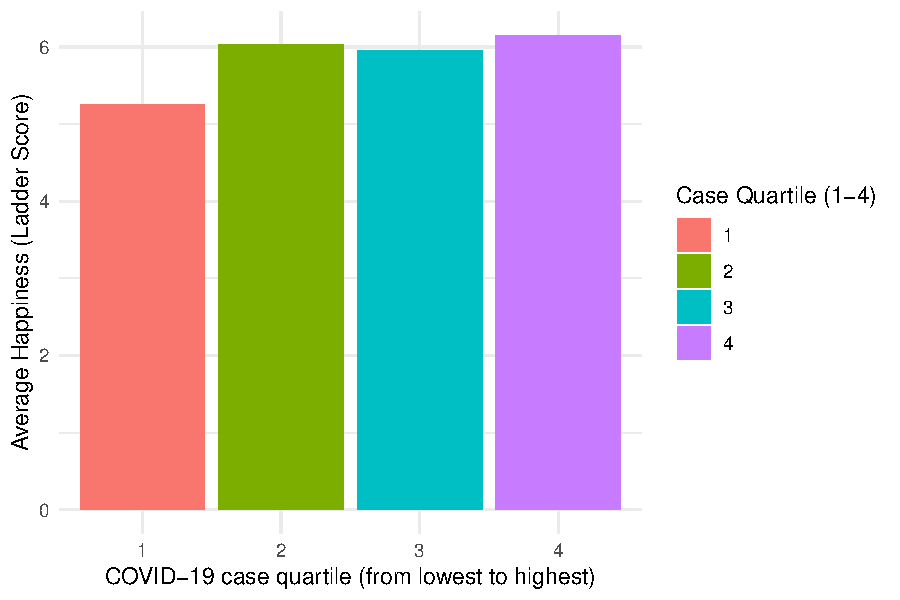
\includegraphics[keepaspectratio]{DATA100Assignment3PartII_Final_Report_Template_files/figure-latex/insight3-1.pdf}}
Countries in the highest COVID-case quartile also report the highest average happiness, which reflects patterns seen in COVID-19 reporting and Life Ladder data \footnote{Ritchie, H., Mathieu, E., Rodés-Guirao, L., Appel, C., Giattino, C., Ortiz-Ospina, E., Hasell, J., Macdonald, B., Beltekian, D., \& Roser, M. (2020). Coronavirus pandemic (COVID-19) {[}Data set{]}. Our World in Data. \url{https://ourworldindata.org/coronavirus}}\footnote{Helliwell, J. F., Layard, R., Sachs, J. D., \& De Neve, J.-E. (2023). World Happiness Report 2023 {[}Data set{]}. Sustainable Development Solutions Network. \url{https://worldhappiness.report}}.

Surprisingly, countries in the highest COVID-case quartile also report the highest average happiness. This counterintuitive pattern can be explained by the fact that regions such as Western Europe, North America, Australia, and parts of East Asia both experienced high reported case counts and consistently rank among the highest on the Life Ladder. In contrast, many countries with limited testing capacity reported fewer cases but also tend to have lower happiness scores. As a result, the association between higher case counts and higher happiness is indirect and largely reflects differences in economic development and infrastructure rather than any meaningful effect of COVID-19 itself.

\section{Conclusion and Future Work}\label{conclusion-and-future-work}

Overall, we found three consistent patterns across the disparate datasets. First, countries with more reported COVID-19 cases tend to show higher levels of climate awareness. This likely reflects stronger education systems, more robust scientific communication, and better reporting capacity in more developed regions. Second, higher climate awareness is associated with higher national happiness, suggesting that climate literacy may be part of a broader set of educational, social, and institutional advantages that contribute to well-being. Third, countries with the highest numbers of COVID-19 cases also rank among the happiest. Rather than indicating any causal relationship, this pattern appears to be driven by differences in economic development: wealthier countries both test more extensively and consistently report higher Life Ladder scores. Together, these findings suggest that global indicators such as public health outcomes, climate awareness, and subjective well-being are interconnected through underlying socioeconomic structures \footnote{The World Bank. (2023). Country and lending groups {[}Data set{]}. \url{https://datahelpdesk.worldbank.org/knowledgebase/articles/906519}}\footnote{United Nations Development Programme. (2023). Human Development Report 2023 {[}Data set{]}. \url{https://hdr.undp.org}}.

For future work, several extensions could strengthen this analysis. Incorporating variables such as GDP, literacy rates, or education indexes would help control for differences in development and allow for a clearer interpretation of the relationships observed \footnote{The World Bank. (2023). Country and lending groups {[}Data set{]}. \url{https://datahelpdesk.worldbank.org/knowledgebase/articles/906519}}\footnote{United Nations Development Programme. (2023). Human Development Report 2023 {[}Data set{]}. \url{https://hdr.undp.org}}. Multiple regression models could be used to distinguish direct from indirect effects across variables. Further work might also explore whether higher climate awareness predicts stronger support for climate policy or behavioral change at the national level. Additionally, explicitly including population size---through metrics like COVID-19 cases per capita---could improve the comparability of countries with very different populations.

This analysis also has several limitations. Measures of climate awareness rely on self-reported survey responses, which may be influenced by sampling quality and respondent honesty. Data inconsistencies, such as mismatched country names, require manual cleaning and may result in the exclusion of some countries. COVID-19 case data are affected by differences in testing capacity, meaning that wealthier countries often appear to have more cases simply because they tested more extensively. Most importantly, the relationships identified are correlational rather than causal; they reflect deeper structural factors rather than direct effects between the variables. Finally, sample sizes vary considerably across countries, which may affect the stability of group comparisons.

Despite these limitations, our findings highlight meaningful and interpretable patterns across global climate literacy, public health outcomes, and well-being. The integration of disparate datasets provides valuable insight into how social, economic, and institutional factors shape international trends in awareness, happiness, and reported health data.

\section{References}\label{references}

\end{document}
